\chapter{Background: Algebraic logic}\label{chap:background3}

\section{Paul Halmos' algebraic logic}

Every Boolean algebra $\mathbb{A}$ is isomorphic to the set of all continuous functions from $X$ into $\mathbb{O}$, where $X$ is the dual space of the algebra $\mathbb{A}$, and $\mathbb{O}$ is the Boolean algebra with 2 elements.  If there is a homomorphism $f$ between Boolean algebras $\mathbb{A} \rightarrow \mathbb{B}$ then there is a dual morphism $f^*$ between their dual spaces $Y \rightarrow X$:
\begin{equation}
\begin{tikzcd}[column sep=3cm, row sep=0.6cm]
\mathbb{A} \arrow[r,"f"] \arrow[d,shift left=2,phantom,"\cong"{anchor=south,rotate=90}] & \mathbb{B} \arrow[d,shift left=2,phantom,"\cong"{anchor=south,rotate=90}] \\
\overbracket{X} \arrow[d] & \overbracket{Y} \arrow[d] \arrow[l,"f^*"] \\
\underbracket{\mathbb{O}} & \underbracket{\mathbb{O}} 
\end{tikzcd}
\end{equation}

\section{Yuri Manin and Russians}

\section{Term rewriting and all that}

\begin{equation}
\vcenter{\hbox{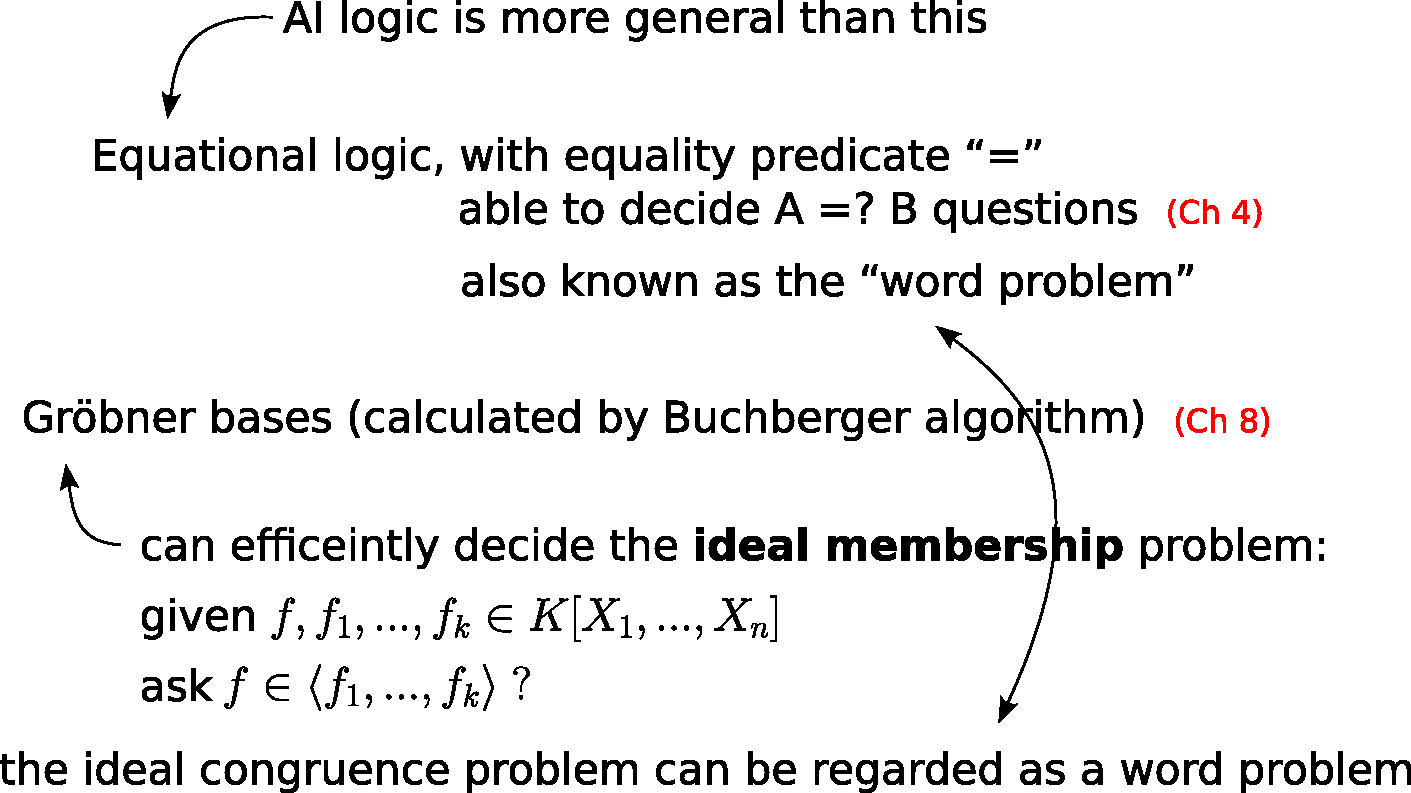
\includegraphics[scale=0.7]{term-rewriting-and-all-that.png}}}
\end{equation}

\begin{itemize}
	\item What is the \textbf{word problem}? \\
	is defined for an equational theory $E$. \\
	is the problem of deciding whether $s = t$
	
	\item why is Gr\"{o}bner basis equivalent to the word problem? \\
	to ask ideal congruence $f =? g$ means $f - g \in? J$ \\
	which is ideal membership problem \\
	a polynomial can be regarded as a rewrite rule \\
	because $f = 0$, we can take the ``largest monomial'' in $f$ as the LHS, and the rest of $f$ as RHS. \\
	In other words:  ideal = set of rules \\
	We ask if a polynomial can be rewritten by the set of rules to another form.  \\
	This is similar to logic deduction.
	
	\item Here an important question is: polynomial reduction seems unable to handle \textbf{logic variables}, it seems only capable of \textbf{simple symbolic rewriting}.
	
	\item logic is equivalent to what form of polynomials? \\
	taking the cue that Huet's higher-order unification = Buchberger algorithm, ...
\end{itemize}

